\chapterpageavan{Avances}
\chapterstar{Avances}

\avancesfigureson                   % <-- Activa el formato especial





En este capítulo se presentan los avances obtenidos durante el desarrollo del sistema de gestión de inventario para la Farmacia Selene. En esta etapa del proyecto se ha trabajado principalmente en la estructuración de la base de datos, el desarrollo del backend y la API, la preparación de los datos iniciales provenientes de los registros de la farmacia, así como la construcción inicial de la interfaz web que permitirá interactuar con el sistema.


\section*{Diseño de la Base de Datos en PostgreSQL}

Uno de los primeros avances del proyecto fue el diseño e implementación de la base de datos que almacena toda la información del sistema. La base de datos fue diseñada siguiendo un enfoque modular, organizando las tablas según su función dentro del sistema. Esta organización permite separar las distintas áreas de información y facilita tanto el mantenimiento como la ampliación futura del sistema.

\begin{figure}[H]
    \centering
    \fbox{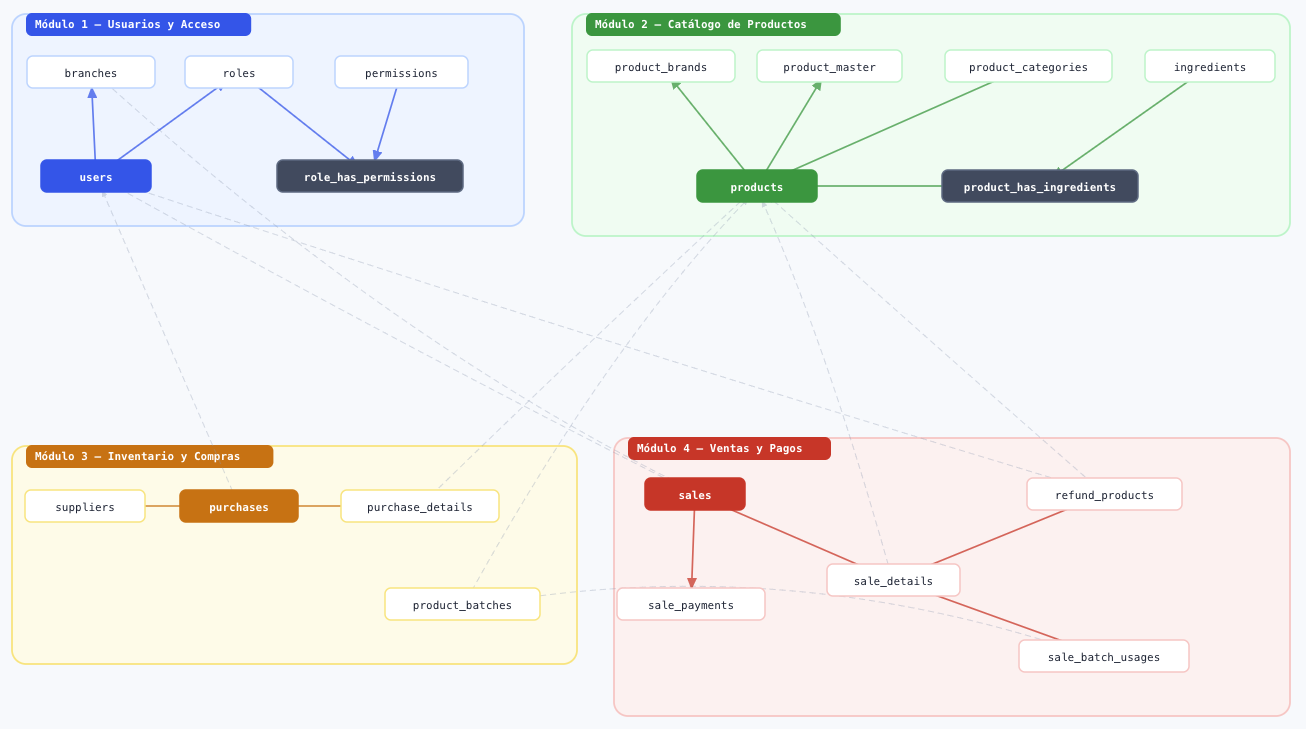
\includegraphics[width=0.9\textwidth]{0_imagenes/Avances1/BDCompleta.png}}
    \caption{Base de datos completa}
    \label{fig:bd-completa}
    
    \vspace{0.2cm}
    \footnotesize \textbf{Fuente:} Elaboración propia.
\end{figure}

Dentro de la estructura de la base de datos se identifican cuatro módulos principales:

\begin{itemize}
\item \textbf{Usuarios y acceso:} gestiona las cuentas del sistema y los mecanismos de autenticación de empleados y administradores.
\item \textbf{Catálogo de productos:} almacena la información básica de los medicamentos y productos disponibles en la farmacia.
\item \textbf{Inventario y compras:} registra las cantidades disponibles de cada producto y los movimientos asociados al abastecimiento.
\item \textbf{Ventas y pagos:} almacena los registros de ventas realizadas y las transacciones correspondientes.
\end{itemize}

\begin{figure}[H]
    \centering
    \fbox{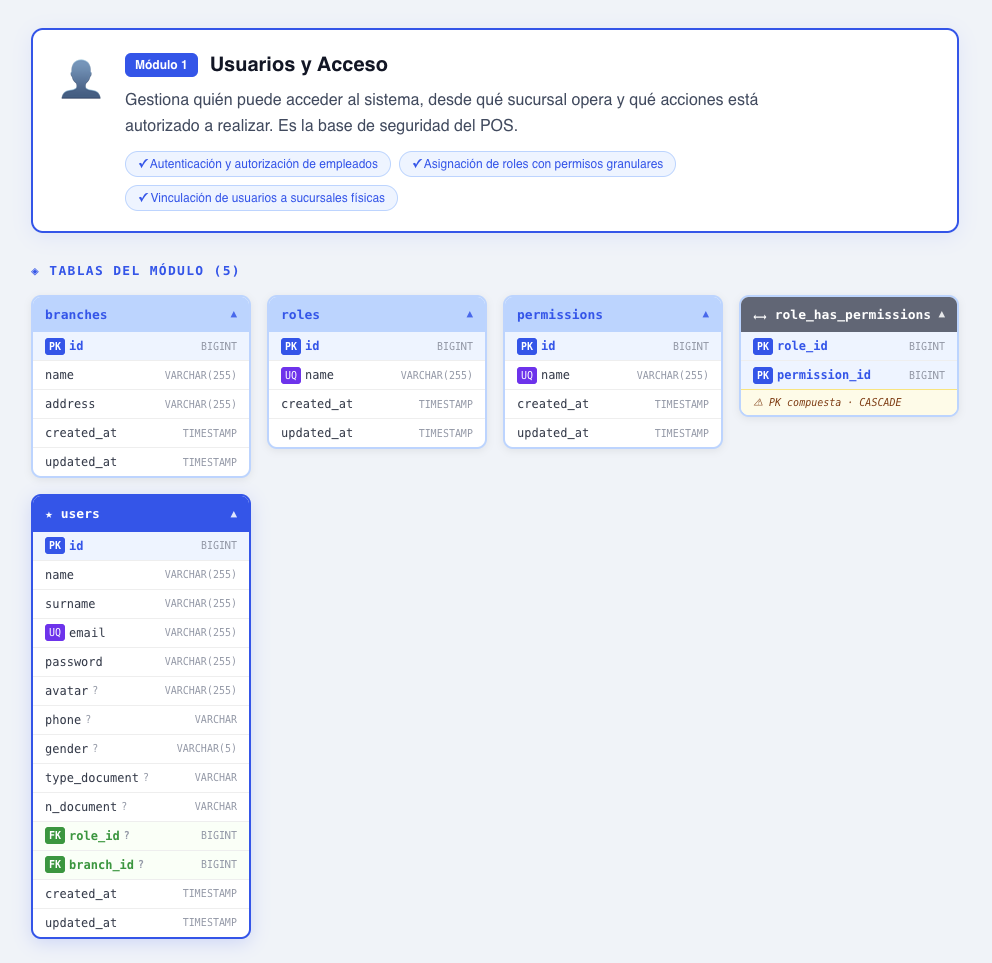
\includegraphics[width=0.5\textwidth]{0_imagenes/Avances1/BDUsuarios.png}}
    \caption{Ejemplo: Modulo de usuarios}
    \label{fig:bd-usuarios}
    
    \vspace{0.2cm}
    \footnotesize \textbf{Fuente:} Elaboración propia.
\end{figure}

Esta estructura modular permite que cada conjunto de tablas cumpla una función específica dentro del sistema, pero manteniendo relaciones entre ellas para asegurar la integridad de la información. Gracias a este enfoque, el sistema puede ampliarse en el futuro mediante la incorporación de nuevos módulos sin necesidad de rediseñar completamente la base de datos.

\section*{Preparación y Limpieza de Datos Iniciales}

Para poblar inicialmente la base de datos se utilizó un archivo de Excel proporcionado por el propietario de la Farmacia Selene, el cual contenía el registro de los productos disponibles en el negocio. Este archivo incluía aproximadamente \textbf{1500 productos}, con información como el nombre del medicamento, su presentación y su precio.

Sin embargo, antes de poder utilizar estos datos dentro del sistema fue necesario realizar un proceso de limpieza y organización de la información. Este tipo de archivos administrados manualmente suele presentar inconsistencias que dificultan su integración directa en una base de datos estructurada.

Durante este proceso se identificaron y corrigieron diversos problemas, entre los que destacan:

\begin{itemize}
\item Registros duplicados de productos.
\item Diferencias en el formato de nombres o descripciones.
\item Información incompleta o mal organizada en algunas columnas.
\end{itemize}

Para solucionar estos inconvenientes se realizó un proceso de depuración de datos en el que se eliminaron duplicados, se normalizaron los nombres de los productos y se reorganizaron los campos de información. Posteriormente, la información fue transformada al formato JSON, un estándar ampliamente utilizado en aplicaciones web modernas para el intercambio estructurado de datos entre sistemas.
\newpage

La Figura \ref{fig:excel-datos} muestra un fragmento del archivo original en Excel, mientras que la Figura \ref{fig:json-datos} presenta la estructura equivalente convertida al formato JSON utilizado por el sistema.

\begin{figure}[H]
    \centering
    \fbox{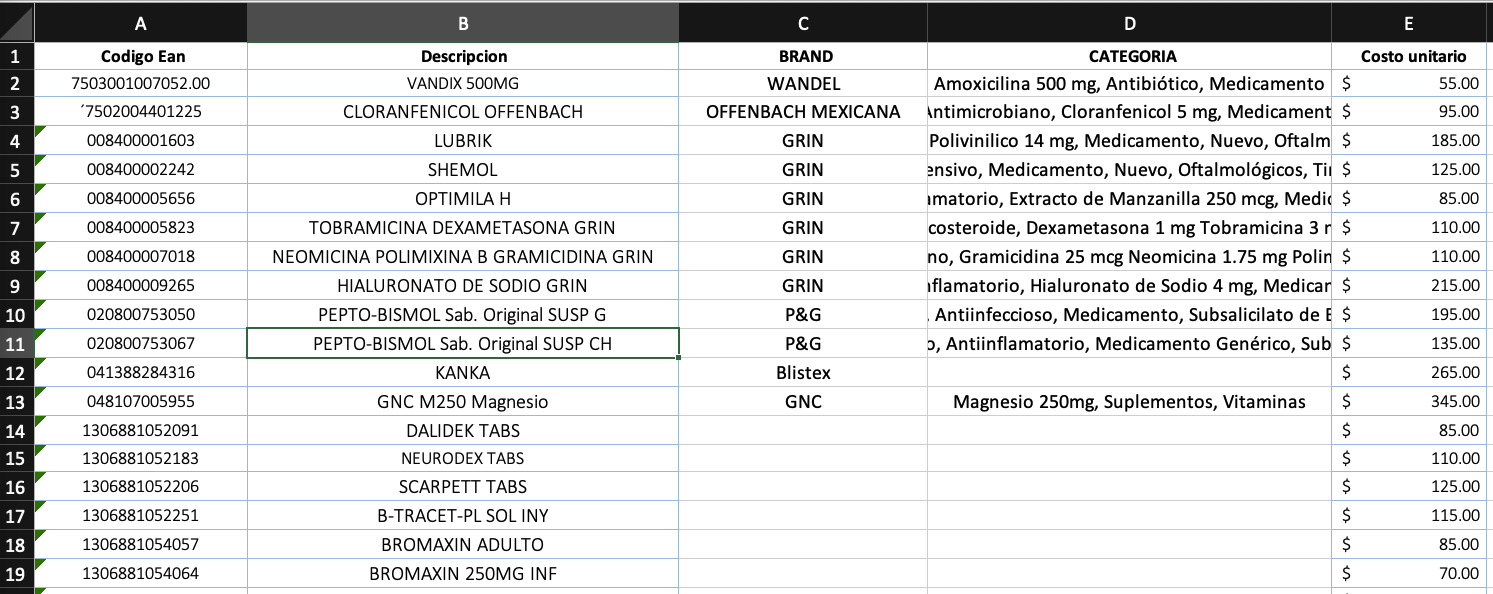
\includegraphics[width=\textwidth]{0_imagenes/Avances1/DatosExcel.png}}
    \caption{Datos originales del catálogo de productos en formato Excel}
    \label{fig:excel-datos}
    
    \vspace{0.2cm}
    \footnotesize \textbf{Fuente:} Elaboración propia.
\end{figure}

\begin{figure}[H]
    \centering
    \fbox{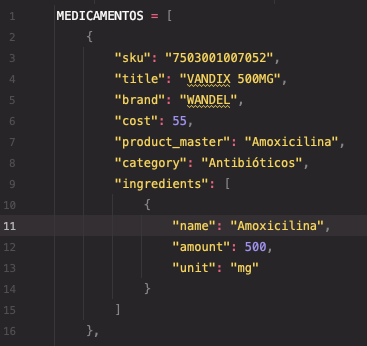
\includegraphics[width=0.5\textwidth]{0_imagenes/Avances1/DatosJSON.png}}
    \caption{Estructura de datos convertida al formato JSON}
    \label{fig:json-datos}
    
    \vspace{0.2cm}
    \footnotesize \textbf{Fuente:} Elaboración propia.
\end{figure}
\newpage

\section*{Desarrollo de la API del Sistema}

Otro de los avances importantes del proyecto fue el desarrollo del backend y la API que permiten la comunicación entre el sistema y las diferentes interfaces que interactúan con él.

La API fue desarrollada utilizando el framework FastAPI y se encarga de procesar las solicitudes del sistema, aplicar las reglas de negocio y gestionar el acceso a la información almacenada en la base de datos.

Actualmente, la API se encuentra desplegada en internet bajo el dominio:

\begin{figure}[H]
    \centering
    \fbox{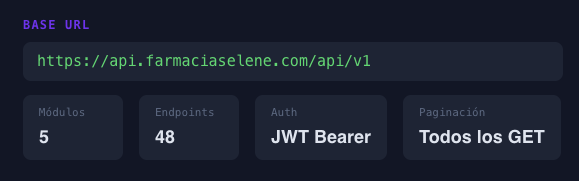
\includegraphics[width=0.8\textwidth]{0_imagenes/Avances1/APIDominio.png}}
    \caption{Dominio público de la API del sistema}
    \label{fig:api-dominio}
    
    \vspace{0.2cm}
    \footnotesize \textbf{Fuente:} Elaboración propia.
\end{figure}

Esto permite que el sistema sea accesible desde cualquier dispositivo autorizado con conexión a internet.

En total, el sistema cuenta con aproximadamente \textbf{48 endpoints}, organizados en distintos módulos funcionales que agrupan las operaciones relacionadas con productos, inventario, usuarios y ventas.

Para garantizar la seguridad en el acceso a la información se implementó un mecanismo de autenticación basado en \textbf{JSON Web Tokens (JWT)}. Este sistema permite que los usuarios autenticados reciban un token temporal que debe enviarse en cada solicitud a la API, asegurando que únicamente usuarios autorizados puedan interactuar con el sistema.

\begin{figure}[H]
    \centering
    \fbox{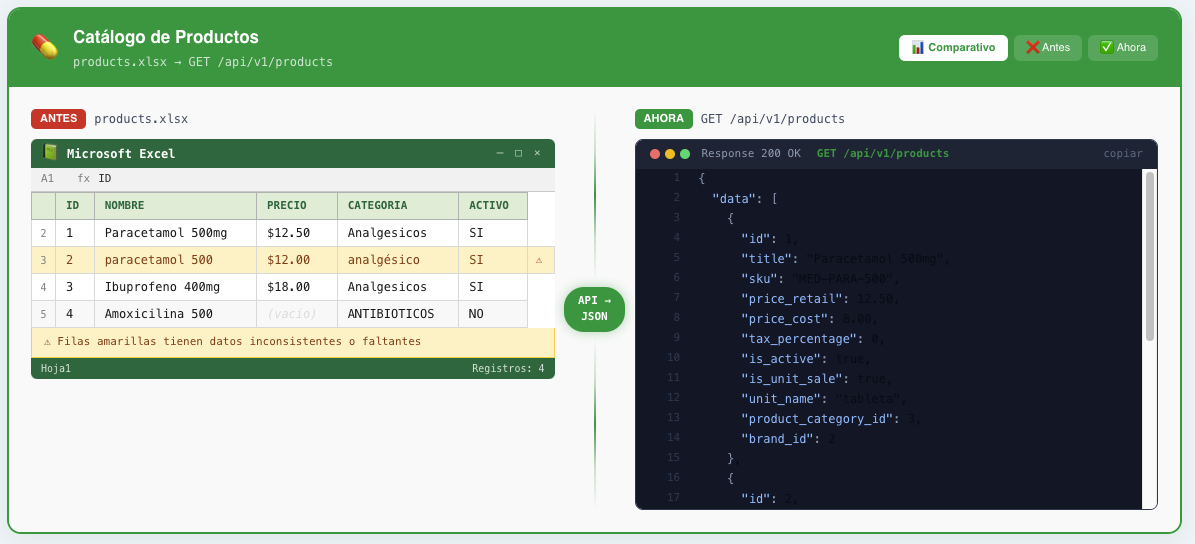
\includegraphics[width=\textwidth]{0_imagenes/Avances1/APIComparativo.png}}
    \caption{Cuadro comparativo}
    \label{fig:api-comparativo}
    
    \vspace{0.2cm}
    \footnotesize \textbf{Fuente:} Elaboración propia.
\end{figure}

\section*{Desarrollo de la Interfaz Web}

Como parte de los avances del proyecto también se inició el desarrollo de la interfaz web del sistema, la cual constituye el medio principal mediante el cual los usuarios interactúan con la plataforma.

Aunque esta interfaz aún se encuentra en proceso de desarrollo, ya permite visualizar y manipular parte de la información almacenada en el backend. A través de la aplicación web, los datos que anteriormente se encontraban distribuidos en distintos archivos de Excel ahora se presentan mediante tablas, formularios y elementos visuales organizados.

Esto permite que los empleados de la farmacia puedan consultar información de productos, revisar el inventario o registrar ventas de manera más clara e intuitiva.

La interfaz web se conecta directamente con la API del sistema para obtener y enviar información en tiempo real. Cada acción realizada por el usuario genera una solicitud al backend, el cual procesa la operación correspondiente y devuelve la respuesta que se muestra en pantalla.

\begin{figure}[H]
    \centering
    \fbox{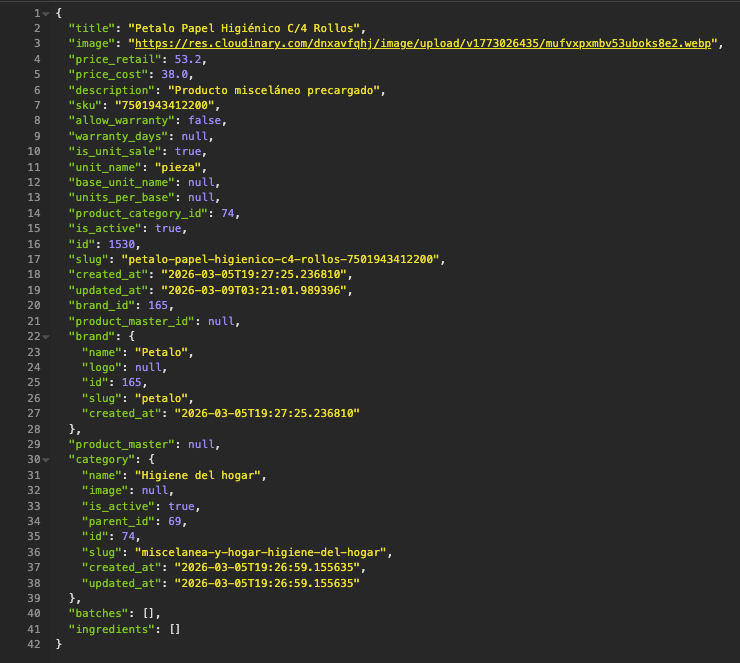
\includegraphics[width=0.6\textwidth]{0_imagenes/Avances1/FRONTENDJSON.png}}
    \caption{Respuesta de la API en formato JSON}
    \label{fig:frontend-json}
    
    \vspace{0.2cm}
    \footnotesize \textbf{Fuente:} Elaboración propia.
\end{figure}

\begin{figure}[H]
    \centering
    \fbox{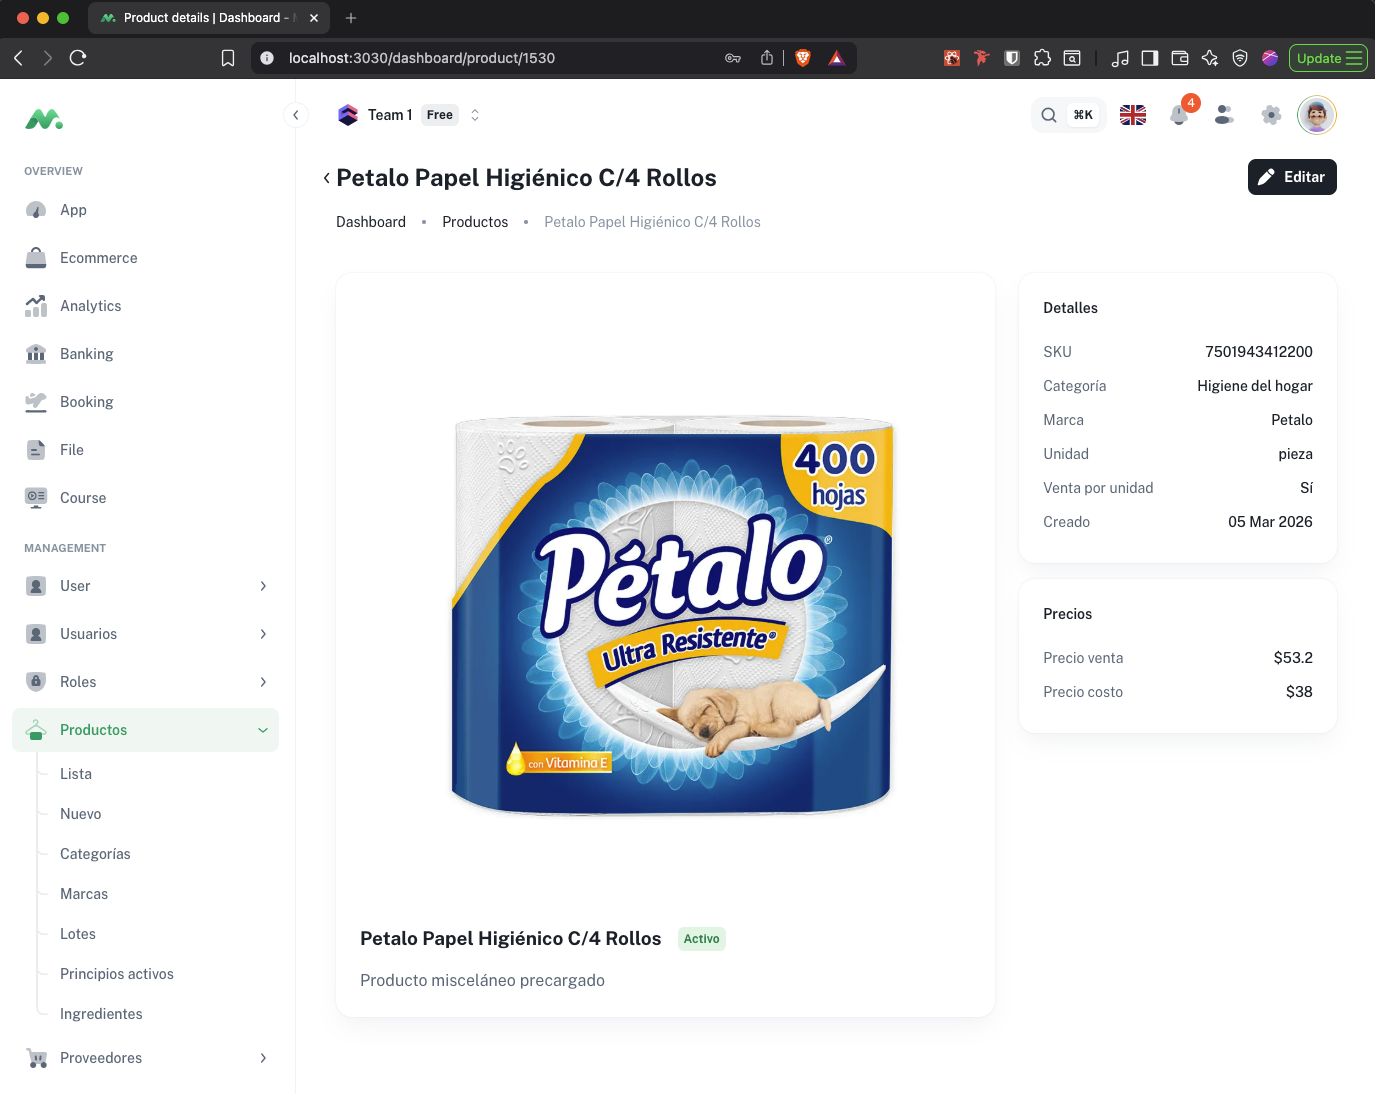
\includegraphics[width=0.7\textwidth]{0_imagenes/Avances1/FRONTENDUI.png}}
    \caption{Interfaz de usuario usando los datos de la API}
    \label{fig:frontend-ui}    
    
    \vspace{0.2cm}
    \footnotesize \textbf{Fuente:} Elaboración propia.
\end{figure}

Los avances descritos en este capítulo representan la base funcional del sistema de gestión de inventario. Actualmente, el backend y la estructura de la base de datos se encuentran operativos, permitiendo el almacenamiento y consulta de información. Asimismo, el desarrollo de la interfaz web continúa en progreso con el objetivo de integrar completamente las funcionalidades del sistema y facilitar su uso dentro de la Farmacia Selene.

% Al finalizar la sección de avances (antes del siguiente capítulo numerado)
\avancesfiguresoff                   % <-- Restaura el formato normal